%\documentclass{article}
\newcommand{\beginsupplement}{%
        \setcounter{table}{0}
        \renewcommand{\thetable}{S\arabic{table}}%
        \setcounter{figure}{0}
        \renewcommand{\thefigure}{S\arabic{figure}}%
     }
\newcommand{\stopsupplement}{%
        \setcounter{table}{0}
        \renewcommand{\thetable}{\arabic{table}}%
        \setcounter{figure}{0}
        \renewcommand{\thefigure}{\arabic{figure}}%
     }

\documentclass[11pt,twoside,lineno]{preprint}
\usepackage{amsmath}
\usepackage[nodisplayskipstretch]{setspace}
\usepackage{makecell} 
\usepackage{changepage}
\setstretch{1.5}
\NeedsTeXFormat{LaTeX2e}
\newcommand*{\articletypename}{PREPRINT}
% Use the documentclass option 'lineno' to view line numbers

% adding commenting commands
\newif\ifcomments
\commentstrue
%\commentsfalse
\newcommand{\cjb}[1]{\ifcomments{{\color{orange} \it (#1)}}\else{}\fi}
\newcommand{\plr}[1]{\ifcomments{{\color{purple} \it (#1)}}\else{}\fi}
\newcommand{\ak}[1]{\ifcomments{{\color{red} \it (#1)}}\else{}\fi}


%Space is the Place: How Dispersal and Competition Shape Genetic Variation in Continuous Space
%Impacts of Continuous Spatial Structure on Analyses of Population Genetic Data
%Impacts of Isolation by Distance on Demographic Modeling and Association Studies
%Space is the Place: How Dispersal and Sampling Shape Inference From Genetic Variation in Continuous Space
%Evolution on the Final Frontier: How Dispersal and Sampling Shape Inference From Genetic Data in Continuous Space
\title{Space is the Place: Effects of Continuous Spatial Structure on Analysis of Population Genetic Data}

\author[$\ast$,1]{C.J. Battey}
\author[$\ast$]{Peter L. Ralph}
\author[$\ast$]{Andrew D. Kern}

\affil[$\ast$]{University of Oregon Dept. Biology, Institute for Ecology Evolution}
\keywords{Space; Population Structure; Demography; Haplotype block sharing; GWAS}

\runningtitle{Effects of Continuous Space} % For use in the footer 

%% For the footnote.
%% Give the last name of the first author if only one author;
% \runningauthor{FirstAuthorLastname}
%% last names of both authors if there are two authors;
% \runningauthor{FirstAuthorLastname and SecondAuthorLastname}
%% last name of the first author followed by et al, if more than two authors.
\runningauthor{Battey \textit{et al.}}

\begin{abstract}
Individuals exist in continuous space, but standard models in population genetics are based on discrete randomly-mating populations. As a result many methods of analyzing genetic data assume that samples are a random draw from a randomly mating population, but are applied to real populations that are structured over space by limited dispersal. Here we implement a forward-time simulation of evolution in continuous space and use it to study the impacts of dispersal and sampling strategy on population genetic summary statistics, demographic inference, and genome-wide association studies. We find that continuous space skews the distribution of several common summary statistics, with the most bias occurring when Wright's neighborhood size is less than 100 and sampling is spatially clustered. In turn estimates of population size history based on the site frequency spectrum become biased in the face of limited dispersal. We show that in the context of genome-wide association studies the combination of spatial variation in the environment and limited dispersal creates spurious signals of genetic association with purely environmental phenotypes across much of the genome and that this bias is only partially corrected by regressing out principal components of ancestry. Last we discuss the relevance of our simulation results for inference from genetic variation in real organisms. 
\end{abstract}

\begin{document}

\maketitle
\thispagestyle{firststyle}
%\marginmark
\firstpagefootnote


\correspondingauthoraffiliation{1}{301 Pacific Hall, University of Oregon Dept. Biology, Institute for Ecology and Evolution. cbattey2@uoregon.edu.}
\vspace{-35pt}% Only used for adjusting extra space in the left column of the first page

\section{Introduction}
The inescapable reality that biological organisms live, move, and reproduce in continuous spatial landscapes has been all but ignored in population genetic models. Indeed, a near universal rule of reproduction is that individuals mate with other nearby individuals, leading to a positive correlation between genetic and geographic distances. This pattern of "isolation by distance" \citep{Wright1943} is one of the most widely replicated empirical findings in population genetics \citep{Chen2017,Jay2012,Sharbel2000}, but classical mathematical models describing it are flawed approximations of the underlying process \citep{Felsenstein1975}.
As a result many studies focus on describing geographic structure as a set of populations connected by migration \citep{Malecot1948,Wright1931}, and analyze variation within clusters of genetic variation inferred by programs like \textit{STRUCTURE} \citep{Pritchard2000} assuming these are randomly mating units. 

Though discrete models of between-population differentiation account for much of the genetic variation in species, the assumption that populations are randomly mating at some level has important implications for downstream inference of selection and demography. Methods based on the coalescent \citep{Kingman1982} assume that the sampled individuals are a random draw from a randomly mating population. If dispersal or mate selection is limited by space these assumptions are violated -- nearby individuals will be more closely related than an average random pair and drawing multiple samples from the same point on the landscape will represent a biased sample of the genetic variation present in the whole population. All downstream inferences drawn from the patterns of relationship inferred among sampled individuals will be subject to bias, but the extent depends on the degree of variation in ancestry across the landscape. 

Our understanding of how many common summary statistics respond to variation in dispersal distance is limited. Tajima's $D$, for example, is often interpreted as reflecting evidence of selection or past population size changes (CITE \cjb{CJ: what's a good citation here?}). However this statistic is essentially a summary of the site frequency spectrum, which itself reflects variation in branch lengths of the underlying genealogy of sampled individuals. Because the spatial extent of dispersal and mate selection determines the rate of drift in a continuously distributed population \citep{Maruyama1972}, these population genetic summaries should also reflect variation in the scale of spatial interactions both over time and across populations. Similarly, the distribution of tract lengths of identity by state among individuals is often interpreted either through the lens of historic demography \citep{Harris2013} or selection \citep{Garud2015}. While that is so this distribution also contains abundant information about dispersal and mate selection \citep{Ringbauer2017,Baharian2016}. We are particularly keen on examining how such summaries will be affected by models that incorporate continuous space. 

A related issue is the spatial distribution of sampling effort. Though individuals in a random-mating population are exchangeable, those in a continuously structured population are not. If sampling is clustered at a series of points on the landscape, as is common in empirical studies because of the practical difficulties of sample collection, samples drawn from a spatially structured population may partially reflect spatial biases in the sampling process rather than in the underlying population. In addition, range edges have been observed to create complex patterns of heterozygosity in stepping-stone simulations \citep{Neel2013,Shirk2014}, but the effects of this process on many downstream inference procedures is unknown. \cjb{must be more out there on sampling -- any recs for papers to read+cite?}

The issue of fine-scale structure for putatively "within-population" analyses may have important implications for genome-wide association studies as well. This is because the genome-wide allele frequency variation caused by isolation by distance is similar to that expected when many sites in the genome are associated with a given phenotype \citep{Bulik-Sullivan2015}. When population structure and the environment covary across space genome-wide association studies (GWAS) may incorrectly infer phenotypic association at many SNPs that have differentiated by drift \citep{Mathieson2012}. This may be a particularly important effect when using GWAS to study selection on polygenic traits. Indeed two recent studies found that previous evidence of polygenic selection on human height in Europe was confounded by subtle population structure \citep{Sohail2018,Berg2018}, suggesting that existing methods to correct for population structure in GWAS are insufficient. However we have little quantitative idea of the population and environmental parameters that can be expected to lead to biases in GWAS. As the scale of sequence data now available for many species allows inference of increasingly fine-scale patterns of selection and demography, understanding how and when subtle spatial structure is likely to bias results is an important task for population genetics.

Here we describe an implementation of an individual-based model in continuous space that incorporates overlapping generations, a Gaussian dispersal kernel, and density-dependent fitness. The model scales to chromosome-scale alignments across tens of thousands of individuals and outputs the full genealogy and recombination history of all final-generation individuals. We use this simulation to test how sampling strategy interacts with isolation by distance to cause systematic variation in population genetic summary statistics typically analyzed assuming discrete population models. We then examine how the fine-scale spatial structures occurring under limited dispersal impact demographic inference from the site frequency spectrum. Lastly we examine the impacts of evolution in continuous space on genome-wide association studies (GWAS) and identify regions of parameter space under which the results from GWAS may be misleading.

\ak{I think we can cut the following paragraph if we just add the last sentence above} 
\cjb{agree - commenting out}
%Last we use our model to study the impacts of isolation by distance in continuous space on genome-wide association studies (GWAS). Variation in ancestry proportions between case and control cohorts is expected to cause inflation of test statistics at SNPs with different allele frequencies among populations \citep{Price2006}. Because most phenotypes are influenced by the environment and environmental factors are often spatially correlated, subtle spatial structure within continuous populations can also deflate $p$ values in GWAS of traits influenced by the environment \citep{Mathieson2012}. Here we simulate both the underlying genealogy and phenotypes of a continuously distributed population and seek to identify regions of parameter space -- i.e. the strength of isolation by distance and the spatial distribution of environmental effects on phenotypes -- in which common methods employed for GWAS are subject to confounding of environmental and genetic effects on phenotypes. 

\section{Materials and Methods}
\label{sec:materials:methods}

\subsection{Modeling Evolution in Continuous Space}
The best-studied approaches to population genetics in continuous space were developed by \cite{Wright1942,Wright1943} and \cite{Malecot1948}, who derived expressions for genetic differentiation in continuous space assuming Poisson distributed numbers of offspring and independent dispersal among individuals. A key finding of Wright's model is that many important aspects of continuous populations can be described in terms of "neighborhood size" -- the number of potential mates for an individual in a given generation, defined as $4\pi\sigma^2d$, where $\sigma$ is the average dispersal distance and $d$ is population density. \cite{Maruyama1972} found that the rate of decline in genetic diversity in a 2-dimensional continuous population approaches the random mating expectation when $d\sigma^2 > 1$, and proposed that this had the important implication that most population genetic expectations for randomly mating populations could be applied to continuously distributed populations with relatively little error. 

Though some aspects of continuous populations are well described by the Wright and Malécot models, \cite{Felsenstein1975} showed that the assumptions of independent dispersal and Poisson distributed offspring that are the basis of these models are incompatible. Over time, a population meeting them will clump into a small number of geographic clusters occupying only a part of the available range. Although real populations are often clumped on landscapes due to factors like varying habitat quality and competition among species, the Wright and Malécot models produce much more extreme clumping than is observed in practice and fail to account for the density-dependent declines in population growth rate that are widely observed in real populations (CITE). 

One method for modeling continuous populations is then to assume the existence of a grid of discrete randomly-mating populations connected by migration, which prevents clustering by forcing all regions to be occupied in every generation. Among many other important results drawn from this class of "lattice" or "stepping stone" models, \cite{Rousset1997} showed that the slope of the a linear regression of genetic differentiation ($F_{st}$) against the logarithm of spatial distance is an estimate of neighborhood size. Though good approximations of continuous structure given high dispersal, these models are not truly continuous, force a uniform realized population density across landscapes, and limit investigation of spatial structure below the level of the deme. An alternative method is to model the geographic spread of ancestry backwards in time through a diffusion approximation -- an approach that has recently made significant progress in modeling both dispersal and demographic parameters \citep{Barton2010,Kelleher2014,Ringbauer2017,Ringbauer2018}.

We took a direct approach to the clustering problem of classical forward-time models by incorporating density dependence into an individual-based model similar to the analytic models developed by Wright and Malécot. By scaling the probability of survival in each timestep to local population density we shift reproductive output towards regions of low-density and prevent populations from clustering. A similar approach was taken previously by \citep{Doebeli2003} who used an individual based model with continuous space and density dependent fitness to study the probability of speciation along continuous environmental gradients. However to our knowledge previous implementations of continuous space models have focused on a small number of genetic loci as the unit of analysis, which limits the ability to investigate the impacts of continuous space on genome-wide genetic variation as is now routinely sampled from real organisms. By simulating chromosome-scale sequence alignments and complete population histories we are able to treat our simulations as real populations and replicate the sampling designs and analyses commonly conducted on real genomic data.
\subsection{A Forward-Time Model of Evolution in Continuous Space}

We implemented our model using the non-Wright-Fisher module in the program SLiM v3.0 \citep{Haller2019}. Each time step consists of three stages: reproduction, dispersal, and competition. To reduce the parameter space we use the same parameter, denoted $\sigma$, to modulate the spatial scale of interactions at all three stages by adjusting the standard deviation of the corresponding Gaussian functions. As in previous work \citep{Wright1943,Ringbauer2017}, $\sigma$ as applied in our dispersal step is approximately equal to the mean parent-offspring distance.  

At the beginning of the simulation individuals are distributed randomly on a continuous landscape. Mates are selected proportional to distances among individuals weighted by a Gaussian function with mean $1/(2\pi\sigma^2)$ and standard deviation $\sigma$. Wright's \cite{Wright1943} "Neighborhood Size", defined as $4\pi\sigma^2 K$ where $K$ is the population density, is then the approximate number of individuals available for mating in our simulation. The number of offspring is drawn from a Poisson distribution with mean $1/L$, where $L$ is the average lifespan. If new offspring are produced, we simulate dispersal by taking two draws from a normal distribution with mean 0 and standard deviation $\sigma$ and adding these to the x and y coordinates of the first parent. 

Density-dependent competition is simulated by adjusting the probability of survival of each individual proportional to the local density of individuals up to a distance $3\sigma$ away, scaled according to the same Gaussian function used for mate selection. Given a per-unit carrying capacity $K$ and average fecundity $F$, the probability of survival $d$ for individual $i$ after adjustment for density is:

\begin{equation}
    d_{i}=min(0.95,\frac{1}{1+\rho*\sum_{i}{G(x)}})
\end{equation}
where 
\begin{equation}
    \rho = F/((1+F)*K)
\end{equation} 
and $G(x)$ is the Gaussian function used to weight distances to other individuals. 

A major challenge in all spatial models is dealing with range edges. When local population density is used to model competition, edge or corner populations can be assigned artificially high fitness values because they lack neighbors within their interaction radius but outside the bounds of the simulation. We approximate a decline in habitat suitability near edges by decreasing the probability of survival proportional to the square root of distance to edges in units of $\sigma$. The final probability of survival for individual \textit{i} is then

\begin{equation}
    s_{i}=d_{i} min(1,\sqrt{x_{i}/\sigma})
    min(1,\sqrt{y_{i}/\sigma})\\
    min(1,\sqrt{(x_{max}-x_{i})/\sigma})
    min(1,\sqrt{(y_{max}-y_{i})/\sigma)}
\end{equation}

where $x$ and $y$ are spatial coordinates. In practice this creates a one $\sigma$ buffer around the edge of the map in which fitness is depressed.

To isolate spatial effects from other components of the model such as overlapping generations, increased variance in reproductive success, and density-dependent fitness, we  also implemented a second version of the SLiM simulation in which mates are selected at random and offspring disperse to a random location on the landscape. We refer to these two models as the "spatial" and "random mating" models. For all simulations the full genealogy and recombination history of final-generation individuals were stored as tree sequences \citep{Kelleher2018}. Scripts for figures and analyses are available at https://github.com/petrelharp/spaceness.  

We ran 400 simulations for the spatial and random-mating SLiM models on a square landscape of size 50 with per-unit carrying capacity $K=5$ (census $N \approx 10,000$), average lifetime $L=4$, genome size $1\times10^{8}$, recombination rate $1\times10^{-9}$, and drawing $/sigma$ values from a uniform distribution bounded by 0.2 and 4. To speed up the simulations and limit memory overhead we used a mutation rate of 0 in SLiM and later applied mutations to the coalesced tree sequence with msprime's 'mutate( )' function. Because msprime assumes that timesteps are in units of generations, we divided the per-generation rate of $1\times10^{-8} mut/site/gen$ by the generation time estimated for each value of $\sigma$ (see 'Genealogical Parameters' below) to convert the rate to units of mutations/site/timestep. We then verified that this procedure produced the correct number of mutations by comparing a subset of simulations with SLiM-generated mutations (which are applied only at mating events) with mutations added by msprime. Simulations were run for 1.6 million timesteps (approximately 30N generations), or until all extant individuals shared a common ancestor within the simulation (i.e. the tree sequence had coalesced). \ak{maybe worth including a table with some basic runtime results in the supplement?}

\subsection{Genealogical Parameters}
Because basic elements of our simulations like census population size and generation time are not directly parameterized in our model (instead they emerge from the interaction of parameters including average population density, average lifespan, and the spatial scale of interaction), we first monitored a range of genealogical parameters in all simulations. We recorded the census population size and estimated the variance in number of offspring and generation time for all simulations. To estimate generation times we stored the age of all parents for 200 timesteps after a 100 generation burn-in and took the mean. To estimate variance in offspring we tracked the number of offspring for all individuals for 100 timesteps following a 100-timestep burn-in period, subset the resulting table to include only the last timestep recorded for each individual, and calculated the variance in number of offspring across all individuals in timesteps 50-100.

\subsection{Sampling}
Our model records the genealogy and sequence variation of the complete population, but in real data genotypes are only observed from a relatively small number of sampled individuals. We modeled three sampling strategies similar to common data collection methods in empirical genetic studies (Figure \ref{fig:samplemap}). "Random" sampling selects individuals at random from across the full landscape, "point" sampling selects individuals proportional to their distance from four equally spaced points on the landscape, and "midpoint" sampling selects individuals in proportion to their distance from the middle of the landscape. Downstream analyses were repeated across all sampling strategies. 


\begin{figure}[htbp]
\centering
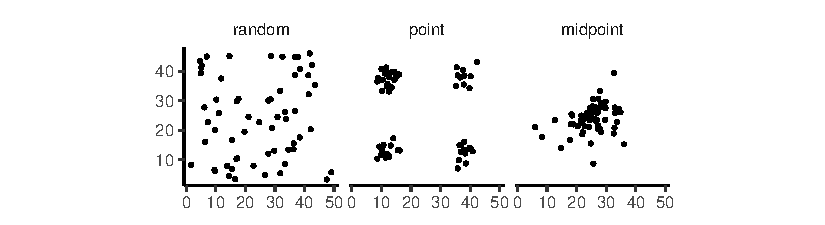
\includegraphics{figures/sampling_maps.pdf}
\caption{Example sampling maps for 60 individuals on a 50x50 landscape under midpoint, point, and random sampling strategies.}
\label{fig:samplemap}
\end{figure}

\subsection{Summary Statistics}
We calculated the site frequency spectrum and a set of 18 summary statistics (Table \ref{table:sumstats}) from 60 diploid individuals sampled from the final generation of each simulation using the python package scikit-allel \citep{Miles2017}. Statistics included common single-population summaries including mean pairwise divergence ($\pi$), inbreeding coefficient ($F_{is}$), and Tajima's D, as well as the classic isolation-by-distance regression of genetic distance ($D_{xy}$) against the logarithm of geographic distances \citep{Rousset1997}, which we summarized as the correlation coefficient between $log10(spatial distance)$ and the proportion of identical base pairs among individuals. 

Following recent studies that showed strong signals for dispersal and demography in the distribution of shared haplotype block lengths \citep{Ringbauer2017,Baharian2016}, we also calculated various summaries of the distribution of pairwise identical-by-state (IBS) block lengths among samples. The full distribution of lengths of IBS tracts for each pair of individuals was first calculated with a custom python function (https://github.com/petrelharp/spaceness/blob/master/scripts/slimtools.py). We then calculated the first three moments of this distribution (mean, variance, and skew) and the number of blocks over $1e6$ base pairs both for each pair of individuals and for the full distribution across all pairwise comparisons. 

We then estimated correlation coefficients between spatial distance and each moment of the pairwise IBS tract distribution. Because more closely related individuals on average share longer haplotype blocks we expect that spatial distance will be negatively correlated with mean haplotype block length, and that this correlation will be strongest (i.e. most negative) when dispersal is low. The variance, skew, and count of long haplotype block statistics are meant to reflect the relative length of the right (upper) tail of the distribution, which represents the frequency of long haplotype blocks so should reflect recent demographic events \citep{Ringbauer2017}. 

The effects of sampling on summary statistic estimates were summarized by testing for differences in mean (ANOVA, \citep{Rcore2018}) and variance (Levene's test, \citep{Fox2011}) across sampling strategies for each summary statistic. 

\subsection{Demographic Modeling}
We fit single-population demographic models to the site frequency spectra of 20 individuals from each spatial SLiM simulation with the program Stairwayplot \citep{Liu2015}. This analysis was replicated across random, point, and midpoint sampling strategies. Site frequency spectra used for input data were calculated in scikit-allel \citep{Miles2017}, and 100 bootstrap replicates were generated for each simulation by resampling over sites. Models were fit across all bootstrap replicates using default settings in Stairwayplot and the median estimate of $Ne$ per generation was used to represent the output of each simulation.

In preliminary runs we found that inferred population histories were relatively variable even when simulating under a coalescent model, suggesting that some of the differences in demographic estimates for spatial models are caused by the behavior of the optimization algorithm rather than bias in the SFS caused by spatial mate choice and dispersal. To separate these effects we ran 100 coalescent simulations with constant population size $6.1\times 10^{-3}$ (the mean $N_{e}$ of random-mating SLiM models estimated from $\Theta_{\pi}$) and fit stairwayplot models using the same script as for our spatial models. All coalescent simulations were performed using msprime \citep{Kelleher2016}. We then calculated the standard deviation of inferred $N_{e}$ in each stairwayplot model to summarize the degree of fluctuation around the simulated population size, and asked if standard deviations were higher in spatial relative to coalescent models with a one-tailed t-test.

\subsection{Association Studies}
To assess the degree to which spatial structure confounds GWAS we simulated four types of nongenetic phenotype variation for 1000 randomly sampled individuals in each spatial SLiM simulation and conducted a linear regression GWAS with PC covariates in PLINK \citep{PURCELL2007}. SNPs with a minor allele frequency less than 0.5\% were excluded from this analysis. Phenotype values were set to vary by two standard deviations across the landscape in a rough approximation of the variation seen in height across Europe, which has recently been found to be confounded with population structure in large scale GWAS \citep{Berg2018,Sohail2018}. Conceptually our approach is similar to that taken in \citep{Mathieson2012}, though here we model fully continuous spatial variation and compare GWAS output across a range of dispersal distances. 

In the first simulation phenotypes for all individuals were drawn from a normal distribution with mean 100 and standard deviation 10.
\begin{equation}
    P \sim \mathcal{N}(100,10)
\end{equation}
Next we simulated clinal environmental influences on phenotype by drawing the phenotypes from independent normal distributions in which the mean was scaled by an individual's x position such that it varied by 2 standard deviations across the map. If $x$ is an individual's x coordinate on a 50x50 landscape, the phenotype is then:
\begin{equation}
    P \sim \mathcal{N}(100+\frac{2x}{5},10)
\end{equation}
Third, we approximate concentrated environmental effects by drawing phenotypes for individuals with x and y coordinates below 20 from a normal distribution with mean 2 standard deviations above the rest of the map. 
\begin{equation}
    P\sim
\begin{cases}
    \mathcal{N}(120,10),& \text{if } x< 20 \text{ and } y<20\\
    \mathcal{N}(100,10),& \text{otherwise}\\
\end{cases}
\end{equation}

Last, we simulated a "patchy" environmental influence on phenotypes by selecting 10 random points on the map and drawing phenotypes for all individuals within two map units of any selected point from a normal distribution with mean 2 standard deviations above the rest of the map. 

\begin{equation}
    P\sim
\begin{cases}
    \mathcal{N}(120,10),& \text{if } d < 3\\
    \mathcal{N}(100,10),& \text{otherwise}\\
\end{cases}
\end{equation}
where $d$ is the distance to the nearest patch. 

Principal components analysis (PCA) was conducted in scikit allel on the matrix of derived allele counts by individual for each simulation. SNPs were first filtered to remove strongly linked sites by calculating LD between all pairs of SNPs in a 200-SNP moving window and dropping one of each pair of sites with an $R^2$ over 0.1. The LD-pruned allele count matrix was then centered and all sites scaled to unit variance when conducting the PCA, following recommendations in \citep{Patterson2006}.   

We ran linear-model GWAS both with and without the first 10 principal components as covariates in PLINK and summarized results across simulations by counting the number of significant SNPs with an expected false positive rate of less than 5\% after adjusting p values with the R function p.adjust(...,method="fdr"). We also examined $p$ values for systemic inflation by estimating the expected values from a uniform distribution (because no SNPs were used when generating phenotypes), plotting observed against expected values for all simulations, and summarizing across simulations by finding the mean $\sigma$ value in each region of quantile-quantile space. Results from all analyses were summarized and plotted with the 'ggplot2' \citep{Wickham2016} and "cowplot" \citep{Wilke2019} packages in R \citep{Rcore2018}. 

\section{Results}

\subsection{Genealogical Parameters}
Having implemented our continuous space forward time population genetic simulation, the first thing we were interested in examining was the effect of spatial parameters on population parameters such as the generation time, the census population size, and the variance in offspring number. In contrast to intuition based on standard population genetic models, in the context of our non-Wright-Fisher model basic quantities like the generation time depend on life history parameters such as the dispersal distance and carrying capacity of the landscape. We first examined how the population size, generation time, and  variance in number of offspring vary with neighborhood size, which itself is a function of $\sigma$ (Figure \ref{fig:genparams}). There are a few things to note. First all three quantities are non-linear with respect to neighborhood size. Census size largely declines as neighborhood size increases for both the spatial and random mating models. However for spatial models this decline only begins for neighborhood size $\geq 10$. By a neighborhood size $\geq 100$ the spatial and random mating models are indistinguishable from one another, a sign that our simulations are performing as expected. Census sizes range from $\approx 14,000$ at low $\sigma$ in the random mating model to $\approx 10,000$ for both models when neighborhood sizes approach 1,000.

\begin{figure}[htbp]
\centering
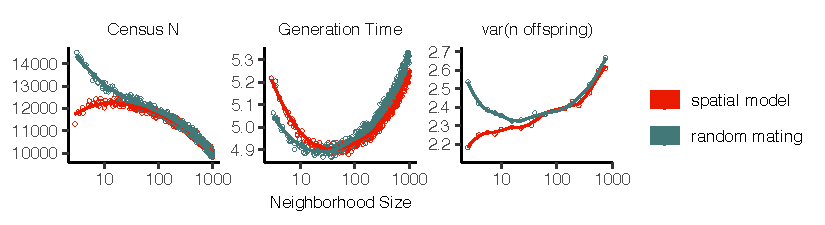
\includegraphics{figures/pop_params.pdf}
\caption{Genealogical parameters from spatial and random mating SLiM simulations, by neighborhood size.}
\label{fig:genparams}
\end{figure}


Generation times similarly show complex behavior with respect to neighborhood sizes, and vary across the parameter range explored between 5.2 and 4.9 timesteps per generation. To stress this point further, the generation time here varies because under our non-Wright-Fisher dynamics individuals are free to reproduce more than once over their lifespan and the lifespan of an individual is only indirectly determined by the parameterization of density-dependent competition the model. Under both the spatial and random mating regimes generation time reaches a nadir at a neighborhood size of $\approx 50$. Interestingly under the range of neighborhood sizes that we examined, generation times between the random mating and spatial models are never quite equivalent -- presumably this would cease to be the case at neighborhood sizes higher than we simulated here.

Last we looked at the effect of neighborhood size on the variance in number of offspring in the population -- a key parameter determining the effective population size. Surprisingly the spatial and random mating model behave quite differently with respect to the neighborhood size: while the variance in offspring number increases monotonically, or nearly so, under the spatial model, the random mating model actually shows a decline in the variance in offspring number until a neighborhood size $\approx 10$ before it increases and eventually equals what we observe in the spatial case. 

%The fitness scaling procedure we use to avoid high fitness at range edges shrinks the suitable area by one $\sigma$ on all sides and likely explains part of the variation in census size, but scaling in offspring variance and the U-shaped distribution of census size in spatial models suggests additional processes at work. For spatial models census size initially rises as neighborhood sizes scale from 2 - 10, which seems to reflect an Allee effect \citep{Allee1949} in which some individuals are unable to find mates when the mate selection radius is very small.  

\subsection{Impacts of Continuous Space on Population Genetic Summary Statistics}
One of the main goals of this study is to examine the effect of continuous space on canonical summaries of population genetic variation. Indeed we have little knowledge to date about how some of our most beloved population genetic summary statistics might be affected by such realistic models. Moreover, as we will show, sampling strategies of individuals with respect to space can affect summaries of variation at least as strongly as the underlying population dynamics. 


\begin{figure*}[p]
\centering
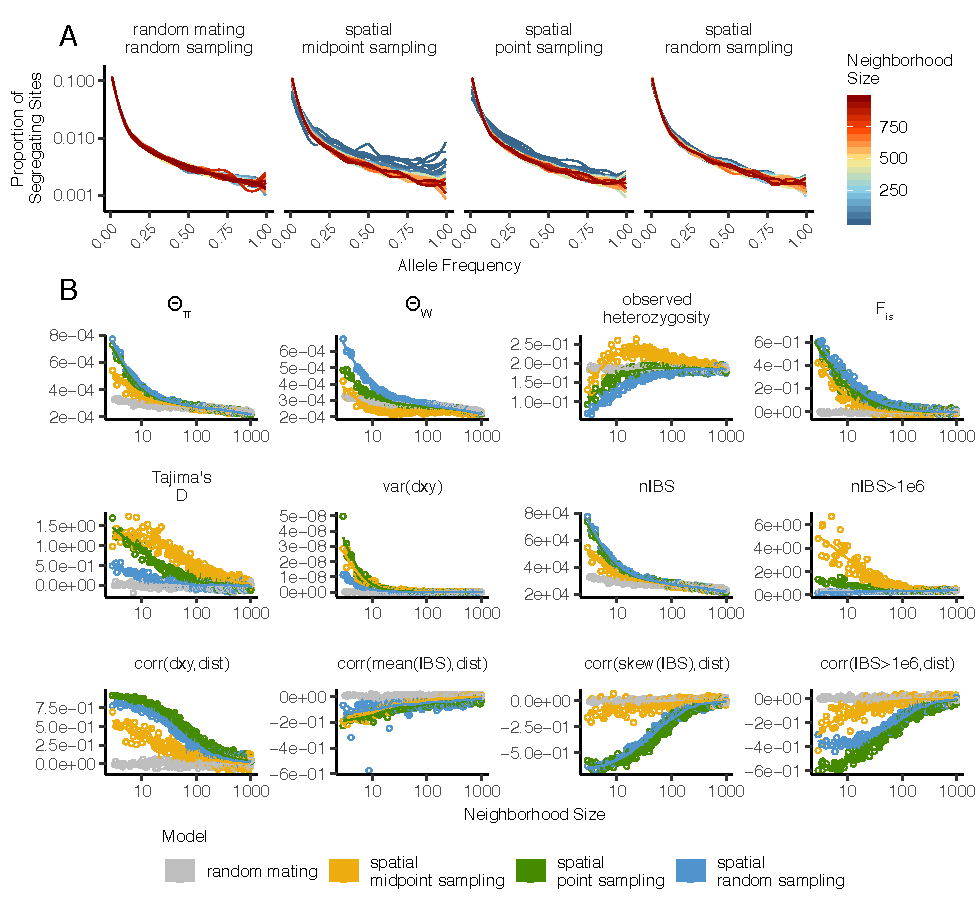
\includegraphics[width=\textwidth]{figures/sfs_w_sumstats.pdf}
\caption{Site frequency spectrum (A) and summary statistic distributions (B) by sampling strategy and neighborhood size.}
\label{fig:sumstats}
\end{figure*}


\subsubsection{Site Frequency Spectra and Summaries of Diversity}
In Figure \ref{fig:sumstats} we examine the effect of varying neighborhood size and sampling strategy on the site frequency spectrum (Figure \ref{fig:sumstats}A) and several canonical population genetic summary statistics (Figure \ref{fig:sumstats}B). For populations in continuous space we observe a significant skew in the SFS for smaller neighborhood sizes ($\leq 100$) that is exacerbated by mid point and point sampling of individuals (see Figure \ref{fig:samplemap}). As expected these effects are strongest for the smallest neighborhood sizes examined and are consistently in the direction of an enrichment of intermediate frequency variants in comparison to the standard neutral expectation. This can be seen succinctly in the response of Tajima's \textit{D} to variation in neighborhood sizes and sampling regime shown in Figure \ref{fig:sumstats}B, whereby we see \textit{D} turning quite positive at small neighborhood sizes. This effect is particularly strong for the midpoint and point sampling regimes, but also occurs under random sampling. Notably, the point at which Tajima's $D$ approaches 0 differs strongly across sampling strategies -- varying from a neighborhood size of $\approx50$ for random sampling to $\geq1000$ for midpoint sampling. 

One of the most commonly used summaries of variation is Tajima's estimator of the neutral mutation rate $\widehat{\theta}_{\pi}$. As can be seen in Figure \ref{fig:sumstats}B $\widehat{\theta}_{\pi}$ can vary as much as nearly three-fold for the smallest neighborhood sizes between the random mating and spatial models depending on the sampling strategies. Each sampling strategy approaches the random mating expectation at its own rate, but by neighborhood size of $\approx 100$ all models are equivalent. These results are to be expected as at small neighborhood sizes the time to the most recent common ancestor for the population should be pushed back-- i.e. it takes longer for lineages to coalesce if dispersal is limited. Interestingly the rate of approach to random mating expectations across sampling strategies is reversed relative to that observed in Tajima's D -- midpoint sampling reaches random mating expectations at neighborhood sizes $\approx50$ while random sampling is inflated until neighborhood size $/approx$ 100. In effect this means that any estimates of population size based on expected heterozygosity from populations with limited dispersal should be treated with caution. 

Patterns from observed heterozygosity and its derivative $F_{is}$ also depend heavily on neighborhood size under spatial models as well as the sampling scheme. $F_{is}$ is inflated above the expectation across most of the parameter space examined and across all sampling strategies. This effect is caused by a deficit of heterozygous individuals in low-dispersal simulations -- a continuous-space version of the Wahlund effect \citep{Wahlund1928}. Indeed for random sampling under the spatial model $F_{is}$ does not approach the random mating equivalent until neighborhood sizes of nearly 1000. The patterns for raw observed heterozygosity are more complex. Under midpoint sampling observed heterozygosity is inflated even over the random mating expectation, as a result of the a higher proportion of heterozygotesn occurring in the middle of the landscape (Figure S\ref{fig:hetmap}). This squares with a report from \cite{Shirk2014} who observed a similar excess of heterozygosity in the middle of the landscape when simulating under a lattice model.

Trends in pairwise haplotype block sharing parallel those in allele-frequency-based diversity estimates (Figure \ref{fig:sumstats}, Supplementary Figure \ref{fig:allsumstats}). At low dispersal the distribution of IBS block lengths in a set of samples is shifted towards smaller values with respect to the random mating expectation-- resulting in lower means and fewer long IBS blocks. The variance and skew of the distribution of haplotype block lengths are only minorly affected by neighborhood size in our simulations when calculated across all pairs of individuals; however, they are strongly dependent on sampling regimes. For example, the number of long haplotype blocks declines as neighborhood size increases under midpoint sampling but changes very little across neighborhood sizes under point or random sampling. Thus sampling strategies with respect to geography will affect conclusions drawn from haplotype length distributions quite dramatically. 

\subsubsection{Correlations of summary statistics with geographic distance}
Correlating population genetic summaries such as $F_{st}$ against geographic distance has shown great utility in empirical population genetics \citep{Rousset1997}. As we know the exact locations of individuals that are sampled in our simulated populations we have examined the relationship of geographic distance among samples with a number of our summary statistics (Figure \ref{fig:sumstats} and Figure \ref{fig:allsumstats}). Starting with a measure of population differentiation,$D_{xy}$, we observe a positive correlation with distance that declines as dispersal increases, as expected under the theory developed by \citep{Rousset1997} and others. This relationship varies across sampling strategies of course, with the weakest correlations observed for midpoint sampling. Moreover there is clearly strong signal for  neighborhood size in the strength of the correlation between $D_{xy}$ and geographic distance.

We next turn our attention to the effect of geographic distance on haplotype block length sharing. As in \citep{Ringbauer2017} and \citep{Baharian2016} we found that the pairwise distribution of haplotype block lengths is more strongly left-skewed under limited dispersal. This is reflected in negative correlation coefficients between spatial distance and the mean, variance, skew, and count of long blocks from the pairwise distribution of identical-by-state block lengths (Figure \ref{fig:sumstats} and Figure \ref{fig:allsumstats}). Of these summaries the mean of the IBS tract length distribution is only weakly affected by neighborhood size, likely because it is heavily influenced by the small number of very long IBS tracts. In contrast the count of long IBS blocks and the skew of the pairwise IBS block distribution are strongly dependent on distance among individuals, and the magnitude of this correlation declines predictably with neighborhood size. In all spatial correlations random and point sampling are similarly correlated with space across neighborhood sizes, but midpoint sampling causes weaker correlations because it incorporates less genetic and geographic distance than the full sample. 

\subsubsection{Effects of Sampling on Random Mating and Spatial Models}
To summarize the effect of sampling strategy on genetic diversity in random mating and spatial models we also asked if summary statistics varied significantly across sampling regimes. In table \ref{table:sampling} we show that for spatial models the mean and variance of nearly all summary statistics was significantly different across sampling strategies (Table \ref{table:sampling}) for spatial models, but not for random mating models. In summary, sampling strategy can be safely ignored when the population is randomly mating but will shape estimates of genetic diversity in any population with limited dispersal. 

\subsection{Effects of Space on Demographic Inference}
One of the most important uses for population genetic data is inferring demographic history of populations. As demonstrated above, the site frequency spectrum varies across neighborhood sizes and sampling strategies. Does this variation lead to different inferences of past population sizes? To ask this we inferred population size histories from samples drawn from our simulated populations using a popular software package that uses the SFS as its information, Stairwayplot \citep{Liu2015}.

In Figure \ref{fig:demography} we show inferred population size histories from our simulations as a function of neighborhood size binned in to one of four categories. In general we observe that demographic models from Stairwayplot tended to infer patterns of ancient population increases and recent declines when neighborhood sizes were below 20 under all sampling strategies (Figure~\ref{fig:demography}). This is consistent with our observations of the SFS from which Stairwayplot is doing its inference. Inflated past population sizes were seen in both point and random sampling, demonstrating that the relatively minor shift in the site frequency spectrum observed among sampling regimes is enough to alter demographic estimates. More alarmingly, inference of severe population bottlenecks was  common at neighborhood sizes under 100 for midpoint and point sampling strategies. Above neighborhood sizes of 100 the average inferred demography across all simulations was relatively accurate, with minor fluctuations slightly above the expected variance $Ne$. While that is so individual model fits were highly variable and often inferred five-fold or greater population fluctuations even in high-dispersal simulations.  
To test whether the variation we observed in inferred demographic histories from Stairwayplot was the result of spatial effects in our simulations rather than the behavior of the optimization routine we compared standard deviations of inferred population sizes in each sampling/neighborhood size bin with those returned by an equilibrium coalescent simulation. Were these to be equal we could assume that the variation were purely as to be expected under the noise inherent in the genealogical process. Instead we found that standard deviations were significantly greater in all sampling strategies for neighborhood sizes under 20 and for midpoint sampling with neighborhood sizes 20-100, but all other sets performed similarly to the coalescent model (Table \ref{table:demography}). In summary, spatial mate choice and dispersal causes strong bias in SFS-based demographic estimates for neighborhood sizes below 20 or when sampling is clustered, but otherwise any biases are within the range of variability regularly inferred by Stairwayplot. This underscores the fact that some \textit{a priori} knowledge about the population dynamics at play will be important to interpreting results of demographic estimation routines. 


\begin{figure}[p]
\centering
\includegraphics[width=\textwidth]{figures/stairwayplot_facet_rollmean.pdf}
\caption{Inferred demographic histories for spatial SLiM simulations from Stairwayplot, by sampling scheme and neighborhood size (NS) range. The thick line is a rolling mean and thin lines are individual model fits. Dashed horizontal lines are the average $N_{e}$ across random-mating SLiM models estimated from $\theta_{\pi}$.}
\label{fig:demography}
\end{figure}

\subsection{GWAS}
To ask what confounding effects spatial genetic variation might have on genome-wide association studies we performed GWAS on our simulations using phenotypes that were determined solely by the environment. In general we found that for simulations with limited dispersal, i.e. neighborhood size $< 100$, spatial variation in the environment causes GWAS to infer significant associations with purely environmental phenotypes at over 25\% of sampled SNPs if no correction for genetic relatedness among samples is performed (Figure \ref{fig:gwas}). This effect is particularly strong for clinal and corner environments, for which the lowest dispersal levels cause over 60\% of SNPs in the sample to return significant associations. Patchy environmental distributions, which result in fewer extreme phenotype values in the sample (Figure \ref{fig:gwas}A), cause fewer false-positives overall but still produce spurious associations at roughly 10\% of sites at the lowest neighborhood sizes. Notably no simulations with nonspatial environments returned more than one significant association (Figure \ref{fig:gwas}C), demonstrating that this effect is caused specifically by the interaction of population structure and spatial variation in the environment rather than by population structure itself.  

When PCA positions are included as covariates to control for population structure in GWAS the vast majority of SNPs no longer surpass a 5\% FDR significance threshold, but up to 1.5\% of SNPs are significantly associated at low dispersal distances under corner and patchy environmental distributions (Figure \ref{fig:gwas}C). At neighborhood sizes $> 500$ up to 0.31\% of SNPs were significant for corner and clinal environments. Given an average of 132,000 SNPs across simulations after MAF filtering, this translates to up to 382 false-positive associations. In most cases the $p$ values for these associations were significant after FDR correction but would not pass the threshold for significance under the more conservative Bonferroni correction, suggesting that the most strongly associated variants from many GWAS of mono- or oligogenic traits are robust to this variety of stratification bias. 

Clinal environments cause an interesting pattern in false positives after PC correction: at low neighborhood sizes the correction removes nearly all significant associations, but at neighborhood sizes above $\approx250$ the proportion of significant SNPs increases to up to 0.4\% (Figure \ref{fig:gwas}. This appears to reflect a loss of descriptive power in the PCA -- as neighborhood size increases, the total proportion of variance explained by the first 10 PC axes declines from roughly 0.1 to 0.04 (Figure \ref{fig:gwas}B). Essentially, PCA seems unable to effectively summarize the weak population structure present in large-neighborhood simulations, but these populations continue to have enough spatial structure to create significant correlations between genotypes and the environment. A similar process can also be seen in the corner phenotype distribution, in which the count of significant SNPs initially declines as neighborhood size increases and then increases at approximately the point at which the proportion of variance explained by PCA approaches its minimum. 

In Figure \ref{fig:gwas}D we present quantile-quantile plots that show the degree of genome-wide inflation of test statistics in PC-corrected GWAS across all simulations and environmental distributions. For clinal environments $-log_{10}(p)$ values are most inflated when neighborhood sizes are large, consistent with the pattern observed in the count of significant associations after PC regression. In contrast corner and patchy environments cause the greatest inflation in $-log_{10}(p)$ at neighborhood sizes $<100$, which likely reflects the inability of PCA to account for fine-scale structure caused by very limited dispersal. Finally, we observed that PC regression appears to cause some degree of overcorrection for all phenotype distributions, visible in Figure \ref{fig:gwas}D as points falling below the 1:1 line.


\begin{figure*}[p]
\centering
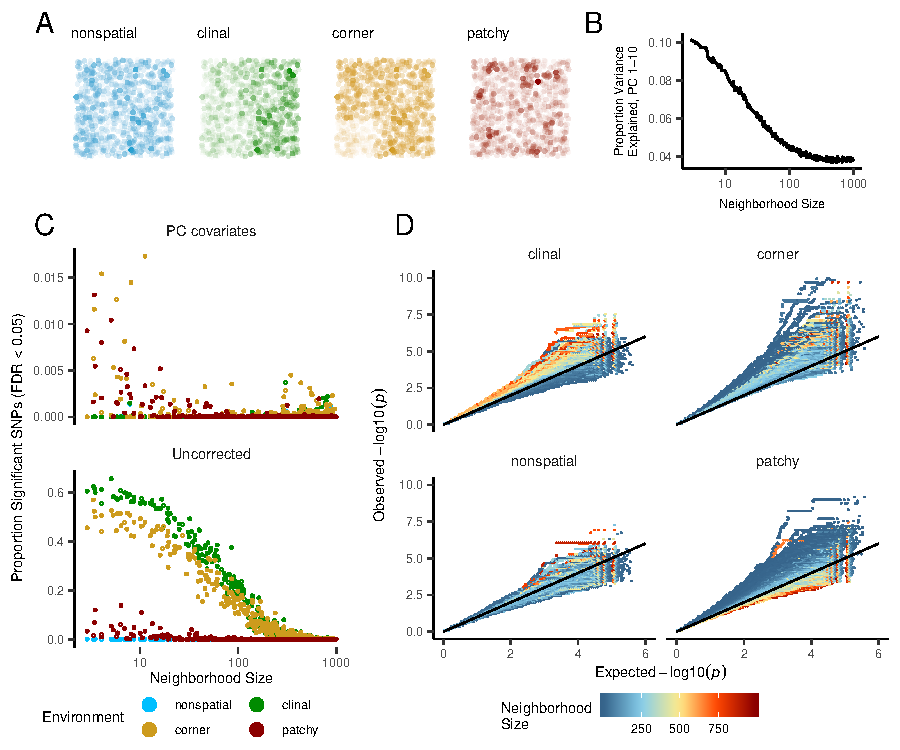
\includegraphics[width=\textwidth]{figures/gwas_summary.pdf}
\caption{Impacts of spatially varying environments and isolation by distance on linear regression GWAS. Simulated quantitative phenotypes are determined only by an individual's location and the spatial distribution of environmental factors. In \textbf{A} we show the phenotypes and locations of sampled individuals under four environmental distributions, with transparency scaled to phenotype. As neighborhood size increases a PCA explains less of the total variation in the data (\textbf{B}). Spatially correlated environmental factors cause false positives at a large proportion of SNPs, which is partially but not entirely corrected by adding PC positions as covariates (\textbf{C}). Quantile-quantile plots in \textbf{D} show inflation of $-log10(p)$ after PC correction across all simulations and environmental distributions, with colors scaled by the median neighborhood size in each region of q-q space.
%A: example environmental distributions and sampling maps, with colors scaled to phenotype values. B: proportion of total variance explained by the first 10 PC axes, by neighborhood size. C: Proportion of significant SNPs after FDR correction for GWAS conducted with (top) or without (bottom) PC covariates. D: Quantile-quantile plots of observed $p$ values relative to those expected from a uniform distribution. The dotted lines show the 95\% confidence region assuming binomial sampling and an alpha level of 0.05. Points above the 1:1 line reflect deflated $p$ values.
}
\label{fig:gwas}
\end{figure*}

\section{Discussion}
Patterns of genetic variation are influenced by the fact that organisms are more likely, on average, to reproduce with others of their species that are geographically proximate, in particular when dispersal distances are short. While historically some analytical progress has been made in describing the influence of continuous space on population genetics (e.g. \cite{Wright1943,Rousset1997,Ringbauer2017,Barton2010}), the theoretical work is challenging and often untenable for realistic biological models. Instead we here use efficient forward time population genetic simulations to describe the myriad influence of space on genetic variation. In particular we examine three axes of variation across three different sampling strategies -- 1) population genetic summary statistics, 2) inference of population size history, and 3) the consequences on genome-wide association studies (GWAS). We are in particular interested in asking how our empirical inferences from data might be affected by spatial processes. As we show below the answers seems to be - often space matters, both because of how populations are sampled with respect to space, and because of the inherent dispersal properties of those populations. 

\subsection{Effects of Dispersal}
Limited dispersal inflates effective population size, creates correlations between genetic and spatial distances, and introduces subtle biases in the site frequency spectrum that are reflected in a positive Tajima's $D$ (Figure \ref{fig:sumstats}). At the extreme low end of dispersal distance this can result in an up to three-fold increase in genetic diversity relative to random-mating expectations. These effects are strongest when neighborhood sizes are below 100, but in combination with the effects of nonrandom sampling they can persist up to neighborhood sizes of at least 1000 (e.g. inflation in Tajima's $D$ and observed heterozygosity under midpoint sampling). Under random sampling the general pattern is similar to expectations of the original analytic model of \cite{Wright1943}, which predicts that populations with neighborhood sizes under 100 will differ substantially from random mating, while those above 10,000 will be nearly indistinguishable from panmixia. 

The patterns observed in sequence data reflect the effects of space on the underlying genealogy. Nearby individuals coalesce rapidly under limited dispersal and so are connected by short branch lengths, while distant individuals take much longer to coalesce than they would under random mating. Mutation and recombination events in our simulation both occur at a constant rate along branches of the genealogy, so the genetic distance and number of recombination events separating two individuals is simply a noisy estimate of the branch lengths connecting them. These genealogical patterns also relate directly to the site frequency spectrum. In our simulations we observed that groups of nearby individuals tend to coalesce rapidly, while coalescence among groups at opposite ends of the landscape takes much longer than under random mating. Tip branches (i.e. branches subtending only one individual) are then relatively short, and branches in the middle of the genealogy connecting local groups of individuals relatively long. These patterns then create the biases we observed in the SFS -- the lowest frequency bins are deflated by the short branch lengths connecting nearby individuals, while mid-frequency bins are inflated by the long branches connecting local groups. 

The genealogical patterns introduced by limited dispersal are particularly apparent in the distribution of haplotype block lengths (Figure \ref{fig:sumstats}). This is because identical-by-state tract lengths reflect the impacts of two processes acting along the branches of the underlying genealogy -- both mutation and recombination -- rather than just mutation as is the case when looking at the site frequency spectrum or related summaries. This means that the pairwise distribution of haplotype block lengths carries with it important information about genealogical variation in the population, and correlation coefficients between moments of the this distribution and geographic location contain signal similar to the correlations between $F_{st}$ or $D_{xy}$ and space \citep{Rousset1997}. Indeed this basic logic underlies two recent studies explicitly estimating dispersal from the distribution of shared haplotype block lengths \citep{Ringbauer2017,Baharian2016}. Conversely, because haplotype-based measures of demography are particularly sensitive to variation in the underlying genealogy, inference approaches that assume random mating when analyzing the distribution of shared haplotype block lengths are likely to be strongly affected by spatial processes. 

\subsection{Effects of Sampling}
One of the most important differences between random mating and spatial models is the effect of sampling: in a randomly mating population the spatial distribution of sampling effort has no effect on estimates of genetic variation, but when dispersal is limited sampling strategy can compound spatial patterns in the underlying genealogy and create pervasive impacts on all downstream genetic analyses. As expected we found that random sampling provides the most accurate summary of genetic diversity across the landscape. However this strategy is often impractical for empirical studies. In reality the difficulty of traveling through all parts of a species range and the inefficiency of collecting single individuals at each sampling site means that most studies follow something closer to the "point" sampling strategy we simulated, in which multiple individuals are sampled from nearby points on the landscape. For example, in ornithology a sample of 10 individuals per species per locality is a common target when collecting for natural history museums. In classical studies of \textit{Drosophila} variation the situation is considerably worse, in which a single orchard might be sampled with bated traps for instance. 

When sampling is clustered at points on a landscape and dispersal is limited, the sampled individuals will be more closely related than a random set of individuals. Average coalescence times of individuals collected at a locality will then be more recent and branch lengths shorter than expected by analyses assuming random mating. This leads to fewer mutations and recombination events occurring since their last common ancestor, causing a random set of individuals to share longer average IBS tracts and have fewer nucleotide differences. For some data summaries, such as Tajima's $D$, Watterson's $\Theta$, or the correlation coefficient between spatial distance and the count of long haplotype blocks, this can result in large differences in estimates between random and point sampling (Figure \ref{fig:sumstats}). Inferring underlying demographic parameters from these summary statistics -- for example, estimating dispersal distance as the slope of a regression of $F_{st}$ against the logarithm of spatial distance \citep{Rousset1997} -- may then be subject to bias if sampling is not random across the landscape. 

However, the largest sampling effects we observed occurred in our "midpoint" sampling strategy. This model is meant to reflect a bias in sampling effort towards the middle of a species' range. In empirical studies this sampling strategy could arise if, for example, researchers choose to sample the center of the range and avoid range edges to maximize probability of locating individuals during a short field season. Because midpoint sampling provides limited spatial resolution it dramatically reduces the magnitude of observed correlations between spatial and genetic distances. More surprisingly, midpoint sampling also leads to strongly positive Tajima's $D$ and an inflation in the proportion of heterozygous individuals in the sample. This increase in observed heterozygosity appears to reflect the effects of range edges, which are a fundamental facet of spatial genetic variation that have often been ignored by analytic approaches focusing on infinite toroidal landscapes \citep{Felsenstein1975}. If individuals move randomly in a finite two-dimensional landscape then regions in the middle of the landscape receive migrants from all directions while those on the edge receive no migrants from at least one direction. The average number of new mutations moving into the middle of the landscape is then higher than the number moving into regions near the range edge, leading to higher heterozygosity and lower inbreeding coefficients ($F_{IS}$) away from range edges. Though here we used only a single parameterization of fitness decline at range edges we believe this is a general property of non-infinite landscapes as it has also been observed in previous studies simulating under lattice models \citep{Neel2013,Shirk2014}. For empirical studies this suggests that sampling only the middle of the landscape will produce a biased view of many aspects of the genetic variation in a population. 

In summary, empirical researchers should collect individuals in as random a manner as practical and should not bias their sample towards the middle of a species' range. When sampling is clustered, summary statistics based on segregating sites (e.g. Watterson's $\Theta$ and Tajima's $D$), heterozygosity, or the distribution of long haplotype blocks, can be expected to depart significantly from what would be observed under random sampling. Comparing the results of analyses conducted on all individuals versus those limited to single individuals per locality may help to reveal any effect of sampling bias if sufficient samples are available. Alternatively, sampling strategy could be incorporated directly into a simulation-based inferential framework by, for example, setting the  distribution of samples in a simulation to mimic that used for the empirical target case. This could be readily achieved in a supervised machine learning or approximate Bayesian setting (CITES).

\subsection{Demography}
Classical population genetic models collapse many elements of life history variation into a single parameter, $N_{e}$, which is then taken to reflect the degree of variation present in the population when modeling the effects of selection or migration. Inferring $N_{e}$ in the past is now a common goal of population genomic analyses and an important step in establishing baseline expectations of genetic variation when searching for signals of selection. Here we found that one method of inference of historic $N_{e}$ based on genome-wide estimates of the site frequency spectrum, Stairwayplot \citep{Liu2015}, is relatively robust to variation in dispersal distance when sampling is random and neighborhood size is over 20. However, non-random sampling, and particularly midpoint sampling, causes the method to infer inflated estimates of past population sizes and a series of recent bottlenecks (Figure \ref{fig:demography}). All sampling strategies lead to inflated ancient and deflated recent $N_{e}$ when neighborhood sizes were less than 20.

These predictions match the biases visible in the raw site frequency spectrum (Figure \ref{fig:sumstats}) -- the deficit of low frequency alleles corresponds to the recent bottlenecks while the inflation of mid-frequency alleles corresponds to the high ancestral $N_{e}$. Though we found that Stairwayplot is a noisy estimator of equilibrium demography in general, there was no significant bias in demographic estimates for any sampling strategy for neighborhood sizes over 100. Thus many existing analyses are likely robust to biases in inferred $N_{e}$ caused by limited dispersal in continuous landscapes. However  barriers to dispersal will likely lead to higher levels of differentiation than we simulated here, and may mimic those seen at the low end of continuous dispersal we simulated.  

\cjb{could be another paragraph here discussing the relationship between Ne, the distribution of coalescence times, and dispersal.}
\ak{wonder if it is worth revisting MSMC or similar now that we know more about how to run the method?}

\subsection{GWAS}
Over the last twenty years genome-wide association studies (GWAS) have identified tens of thousands of correlations between genetic variation and phentoypes, both in humans and other species. This technique is increasingly applied to questions of human health through methods like polygenic risk scores that sum the effect sizes estimated from GWAS to predict an individual's phenotype or disease risk \citep{Khera2018}. The most common approach to GWAS, which we followed in our analyses of simulated data here, is to regress the count of derived alleles at a site against individual phenotypes, taking the slope of this regression as an estimate of the effect of the allele on the phenotype. As recently reviewed by \cite{Visscher2019}, this is exactly the approach outlined by \cite{Fisher1918} at the dawn of quantitative genetics. 

Stepping back from the mechanics of GWAS specifically, the approach of quantitative genetics is to decompose the variance in phenotypes into environmental and genetic effects, e.g. 
\begin{equation}
P=G+E
\end{equation}
\begin{equation}
var(P)=var(G)+var(E)+cov(G,E)
\end{equation}
For GWAS in structured populations, the bias identified in many previous studies \citep{Price2006,Yu2006,Young2018,Mathieson2012,Kang2008,Kang2010,Bulik-Sullivan2015} in which test statistics reflect population structure rather than phenotype association arises because of the presence of a positive covariance between genotypic and environmental variation (the third term above). When the environment and genotype covary across space their effects are confounded. Note this does not require interaction between genotype and environment (so-called GxE effects), which will introduce an additional source of bias. Here we refer simply to the fact that the allele frequency at a site will often covary with the environment when both breeding structure and the environment vary over space. To some degree the success of quantitative genetics in fields like agriculture is likely due to the absence of this covariation -- crop and animal breeding operations can be conducted so that the environment is identical (or nearly so) or randomized across populations. However in natural populations this situation is extremely unlikely. Most populations are structured by a combination of limited dispersal and geographic barriers, and nearly all environments vary over space. GWAS in natural populations is forced to confront the confounding effects of population structure and the environment directly. 

Incorporating PC positions as covariates in the analysis \citep{Price2006} is designed to address this difficulty by regressing out a baseline level of "average" differentiation. However while this approach is quite useful, it does not truly separate the confounding signals of environment and spatially varying genotypes. In essence with a PC-corrected GWAS we are asking "what regions of the genome are more associated with this phenotype than the average genome-wide association observed across populations?" In our simulations we observed that this procedure can fail under a variety of circumstances. If dispersal is limited and environmental variation is clustered in space (i.e. corner or patchy distributions in our simulations), PCA positions fail to capture the fine-scale spatial structure required to remove all signals of association. Conversely when dispersal is high we found that PCA loses power to describe population structure before the spatial scale of dispersal breaks down the relationship between genotype and the environment. These effects were observed in all spatially varying environmental distributions, but were particularly pronounced for concentrated environmental effects in one region, as was also found in \cite{Mathieson2012}. As a result we can expect to see several thousand weak false-positive associations in a PC-corrected GWAS conducted on a human-sized genome in species with neighborhood sizes up to at least 1000. 

This does not mean that GWAS is not useful, but does put some limits on the extent of valid interpretation. Very few of the associations we identified would be significant at a conservative Bonferroni-adjusted $p$-value cutoff, suggesting that most of the very strong signals of association signals observed in studies of mono- or oligogenic traits are robust to stratification bias. Further, the most dramatic effects of stratification inflation we observed occurred at neighborhood sizes below 100 -- smaller than the vast majority of modern human populations (but see below for further discussion of empirical cases). However, as recently identified in studies of gentoype associations for human height in Europe \citep{Berg2018,Sohail2018}, PC regression GWAS in modern human populations does leave residual signal of population structure in large-scale GWAS of polygenic traits. Indeed, studies in strongly structured species like \textit{Arabadopsis} have long relied on more sophisticated mixed model approaches to correcting for population structure for precisely this reason \citep{Aranzana2005,Sasaki2015}.

A second point that has received less attention in the literature is the issue of overcorrection in GWAS. If a truly causal allele segregates at different frequencies in different populations, then correcting for population structure in a regression analysis will result in an underestimate of effect sizes. Though our simulations had no causal alleles, we observed some evidence of this effect in the distribution of $p$-values across the genome (Figure \ref{fig:gwas}D): after PC regression many analyses resulted in $p$-values falling below their expected values from a uniform distribution. This result is consistent with a recent empirical study of heritability in human height and body mass index, which found that increasing the number of PC axes used as covariates caused the total proportion of variance explained by SNPs to decline from $\approx0.8$ to $\approx0.75$ \citep{Wainschtein2019}. Indeed SNPs with minor alleles frequencies of 0.001 - 0.01, which are expected to reflect fine scale population structure \citep{Mathieson2012,Novembre2009}, are estimated to explain \textit{negative} proportions of the total phenotypic variance in \citep{Wainschtein2019}\ak{i don't understand what the authors mean here-- how can we have a negative variance?}. Searching for genetic associations of polygenic traits that vary systematically across but not within populations through existing GWAS approaches is then unlikely to be successful: the signals are fully confounded, and new analytic methods or experiments controlling for variation in the environment will be necessary to rigorously identify causal variants. 

In summary, spatial covariation in population structure and the environment confound the interpretation of GWAS $p$-values, and correction using principal components is insufficient to fully separate these signals for polygenic traits under a variety of environmental and population parameter regimes. How more sophisticated mixed-model methods would perform under our simulations is an interesting question that we plan to pursue in a future study, but statistical methods can only take us so far in the absence of controlled environments. One currently popular approach to estimating the degree of bias in GWAS caused by population structure is LD score regression \citep{Bulik-Sullivan2015}. Though this approach appears to work well in practice, its interpretation is not always straightforward and it is likely biased by the presence of linked selection \citep{Berg2018}. We suggest a straightforward alternative for species in which the primary axes of population differentiation is space (note this is likely not the case for many modern human populations): run a GWAS with spatial coordinates as phenotypes and check for $p$-value inflation or significant associations. If significant associations with sample locality are observed after correcting for population structure through PC regression or a kinship matrix, the structure corrections are insufficient. This is essentially the approach taken in our "clinal" model (though we also include normally distributed variation in our phenotypes). Of course it is possible that genotypes indirectly affect individual locations by adjusting organismal fitness and thus habitat selection across spatially varying environments, but we believe that this hypothesis should be tested against a null of stratification bias inflation rather than accepted as true based on GWAS results.  \cjb{what do you think of the second half here?}

% latex table generated in R 3.5.1 by xtable 1.8-3 package
% Thu Apr 11 13:11:59 2019
\begin{table}[hbpt]
\small
\begin{adjustwidth}{-.9cm}{}
\centering
\caption{\bf Neighborhood size estimates from empirical studies.}
\begin{tabular}{rllrrll}
  \hline
 Species & Description & \makecell[l]{Neighborhood\\Size} & Method & Citation \\ 
  \hline
  \makecell[l]{\textit{Ipomopsis}\\\textit{aggregata}} & flowering plant & 12.60 - 37.80 & Genetic & \citep{Campbell1992}\\
  %\makecell[l]{\textit{Linanthus}\\\textit{parryae}} & flowering plant & 14 - 27 & Genetic & \citep{Wright1943}\\ %this one got debunked by a series of studies in the 90's that found that spatial differentiation in flower color is driven by environmental variability across years. See https://doi.org/10.1111/j.1558-5646.2007.00219.x
  \makecell[l]{\textit{Borrichia}\\\textit{frutescens}} & salt marsh plant & 20 - 30 & Genetic+Survey & \citep{Antlfinger1982} \\ 
  \makecell[l]{\textit{Oreamnos}\\\textit{americanus}} & mountain goat & 36 - 100 & Genetic & \citep{Shirk2014} \\ 
  \makecell[l]{\textit{Homo sapiens}} & \makecell[l]{Gainj- and Kalam- \\speaking people,\\Papua New Guinea} & 40 - 213 & Genetic & \citep{Rousset1997}\\ 
  \makecell[l]{\textit{Formica sp.}} & colonial ants & 50 - 100 & Genetic & \citep{Pamilo1983} \\ 
  \makecell[l]{\textit{Astrocaryum}\\\textit{mexicanum}} & palm tree & 102 - 895 & Genetic+survey & \citep{Eguiarte1993} \\ 
  \makecell[l]{\textit{Spermophilus}\\\textit{mollis}} & ground squirrel & 204 - 480 & Genetic+Survey & \citep{Antolin2001}\\
  \makecell[l]{\textit{Sceloperus}\\\textit{olivaceus}} & lizard & 225 - 270 & Survey & \citep{Kerster1964} \\ 
  \makecell[l]{\textit{Dieffenbachia}\\\textit{longispatha}} & \makecell[l]{beetle-pollinated\\colonial herb} & 227 - 611 & Survey & \citep{Young1988} \\ 
  \makecell[l]{\textit{Homo sapiens}} & \makecell[l]{Gainj- and Kalam- \\speaking people,\\Papua New Guinea} & 410 & Survey & \citep{Rousset1997} \\ 
  \makecell[l]{\textit{Quercus}\\\textit{laevis}} & Oak tree & $>440$ & Genetic & \citep{Berg1995} \\ 
  \makecell[l]{\textit{Drosophila}\\\textit{pseudoobscura}} & fruit fly & 500 - 1,000 & Survey+Crosses & \citep{Wright1946} \\ 
  \makecell[l]{\textit{Homo sapiens}} & \makecell[l]{POPRES data\\NE Europe} & 1,342 - 5,425 & Genetic & \citep{Ringbauer2017} \\ 
  \makecell[l]{\textit{Bebicium}\\\textit{vittatum}} & intertidal snail & 240,000 & Survey & \citep{Rousset1997}\\ 
  \makecell[l]{\textit{Bebicium}\\\textit{vittatum}} & intertidal snail & 360,000 & Genetic & \citep{Rousset1997}\\ 
   \hline
\end{tabular}
\label{table:NStable}
\end{adjustwidth}
\end{table}

\subsection{Where are natural populations on this spectrum?}
For how much of the tree of life do spatial patterns circumscribe genomic variation? In Table \ref{table:NStable} we gathered estimates of neighborhood size from a range of organisms to get an idea of how likely dispersal is to play an important role in patterns of variation. Though this sample is almost certainly biased towards small-neighborhood species (because few studies have quantified neighborhood size in species with very high dispersal or population density), we find that neighborhood sizes in the range we simulated are fairly common across a range of taxa. At the extreme low end of empirical neighborhood size estimates we see some flowering plants, large mammals, and colonial insects like ants. Species such as this have neighborhood size estimates small enough that spatial processes are likely to strongly influence inference. These include some human populations such as the Gainj- and Kalam-speaking people of Papua New Guinea, in which the estimated neighborhood sizes in \citep{Rousset1997} range from 40 to 410 depending on the method of estimation. Many more species occur in a middle range of neighborhood sizes between 100 and 1000 -- a range in which spatial processes play a minor role in our analyses under random spatial sampling but are important when sampling of individuals in space is clustered. Last, many species likely have neighborhood sizes much larger than we simulated, including modern humans in NE Europe \citep{Ringbauer2017}. For these species demographic inference and summary statistics are likely to reflect minimal bias from spatial effects as long as dispersal is truly continuous across the landscape. While that is so we caution that association studies in which the effects of population structure are confounded with spatial variation in the environment are still sensitive to dispersal even at these large neighborhood sizes.

\subsection{Future Directions and Limitations}
As we have shown, a large number of population genetic summary statistics contain information about spatial population processes. We imagine that combinations of such summaries might be sufficient for the construction of supervised machine learning regressors (e.g. \cite{Schrider2018}) for the accurate estimation of dispersal from genetic data. Indeed \cite{Ashander2018} found that inverse interpolation on a vector of summary statistics provided a powerful method of estimating dispersal distances. Expanding this approach to include the haplotype-based summary statistics studied here and applying machine learning regressors built for general inference of nonlinear relationships from high-dimensional data may allow precise estimation of spatial parameters under a range of complex models. 

One complication in the inference of any spatial demographic parameter is the balance between local and global process. Many species are structured locally by limited dispersal, but also contain deeply divergent lineages in different regions that reflect signals of ancient episodes of geographic isolation or strong barriers to dispersal. Gene flow upon secondary contact of two previously isolated lineages should create clinal patterns similar to isolation by distance, and it will be difficult to determine when inferred dispersal parameters are reflecting recent demographic process versus the historic patterns of geographic isolation. In addition, spatially varying selection will create allele frequency variation over space that may mimic isolation by distance. Indeed, a series of field studies described in \cite{Schemske2007} found that in Wright's original empirical example of isolation by distance, the flowering plant \textit{Linanthus parryae}, patterns of flower color differentiation over space primarily reflect temporal and spatial variation in selection rather than limited dispersal. Studies simulating selection and dispersal interacting in space (e.g. \cite{Ralph2010}) and testing for identifiability of inferred dispersal or selective parameters may offer new insight into the extent of our ability to accurately infer evolutionary processes in real systems. 

%Recent methods that aim to estimate geographic barriers to dispersal \citep{Ringbauer2018,Petkova2015} partially address this issue by attempting to infer the location of regions resistant to gene flow, but here again the balance between historical and current demographic processes represented in our inference is unclear. Limiting analyses to low-frequency alleles \citep{Novembre2009} or between long haplotype blocks \citep{Ringbauer2017} is one approach to limiting inference to recent demography (because these genomic features should arise primarily from patterns in the most recent branches of the genealogy), but as we showed spatial processes also cause shifts in branch lengths throughout the genealogy. Further studies on the ways in which the sample genealogy responds to variation in dispersal both over time and across space are a good direction for future research. 

Though our continuous space simulation allows incorporation of realistic demographic and spatial processes and is much faster than previous individual-based models, it is inevitably limited by the computational burden of tracking tens of thousands of individuals in every generation. In particular the calculations required for our mate selection and competition steps involve summarizing distances across all pairs of individuals and so scale very poorly \ak{how exactly does this scale? $O(N^2)$?} as the number of individuals within a three-$\sigma$ radius increases. In part the issue of runtime scaling is a function of the spatial process itself -- under very limited dispersal we observed that coalescence requires over 30N generations, so forward-time methods must be run for a very long time to create a complete genealogy as underlies all real genome sequence data. The reverse-time model of continuous space evolution described in \cite{Barton2010} and implemented in \cite{Kelleher2014} may allow exploration of parameter regimes with population and landscape sizes more directly comparable to empirical cases like humans. However, incorporating selection or other processes into such models will be difficult. 

A mixed approach may be possible by combining forward- and reverse-time models, as was recently done for a continuous-space Wright-Fisher model in \cite{Lotterhos2019} and for a simulation with linked selection in \cite{Buffalo2019}. This would allow us to generate short runs of complex, realistic simulations in forward time in SLiM \citep{Haller2019} and then "finish" the simulations as a coalescent simulation in msprime \citep{Kelleher2016}. However a significant difficulty in this "recapitation" approach is scaling the variance in reproductive output and generation time across forward- and reverse-time methods. Further development of our understanding of how to merge forward- and reverse-time models is a promising avenue for future research that will be necessary for scaling continuous-space simulations to millions or billions of individuals.  

Finally we believe that the difficulties in correcting for population structure in continuous populations using principal components analysis or similar decompositions is a difficult issue, well worth considering on its own -- what does it mean to correct for population structure in a world without discrete demes? What are the boundaries between proper corrections between ancestry and underpowering the search for local genetic variation? We posit that there is progress yet to be made in deriving either process driven descriptions of ancestry or more generalized unsupervised methods that can better account for shared relatedness, say in the context of GWAS, for populations that are structured over space. 
\ak{this paragraph is a bit out there. rein me in}


\section{Data Availability}
Scripts used for all analyses and figures are available at https://github.com/petrelharp/spaceness. 

\section{Acknowledgements}
We thank folks for reading and thinking about this manuscript. We thank the Hearth for having such good nearby coffee. Falling Sky Brewing was key to the success of this research endeavor. CJB and ADK were supported by NIH award R01GM117241. 

\bibliography{spaceness}



%%%%%%%%%%%%%%%%%%%%%%%%%%%%%%%%%%%%%% Supplement %%%%%%%%%%%%%%%%%%%%%%%%%%%%%%%%%%%%%%%
\section{Supplementary Figures and Tables}
\beginsupplement

\afterpage{\clearpage}
\begin{figure*}[p]
\centering
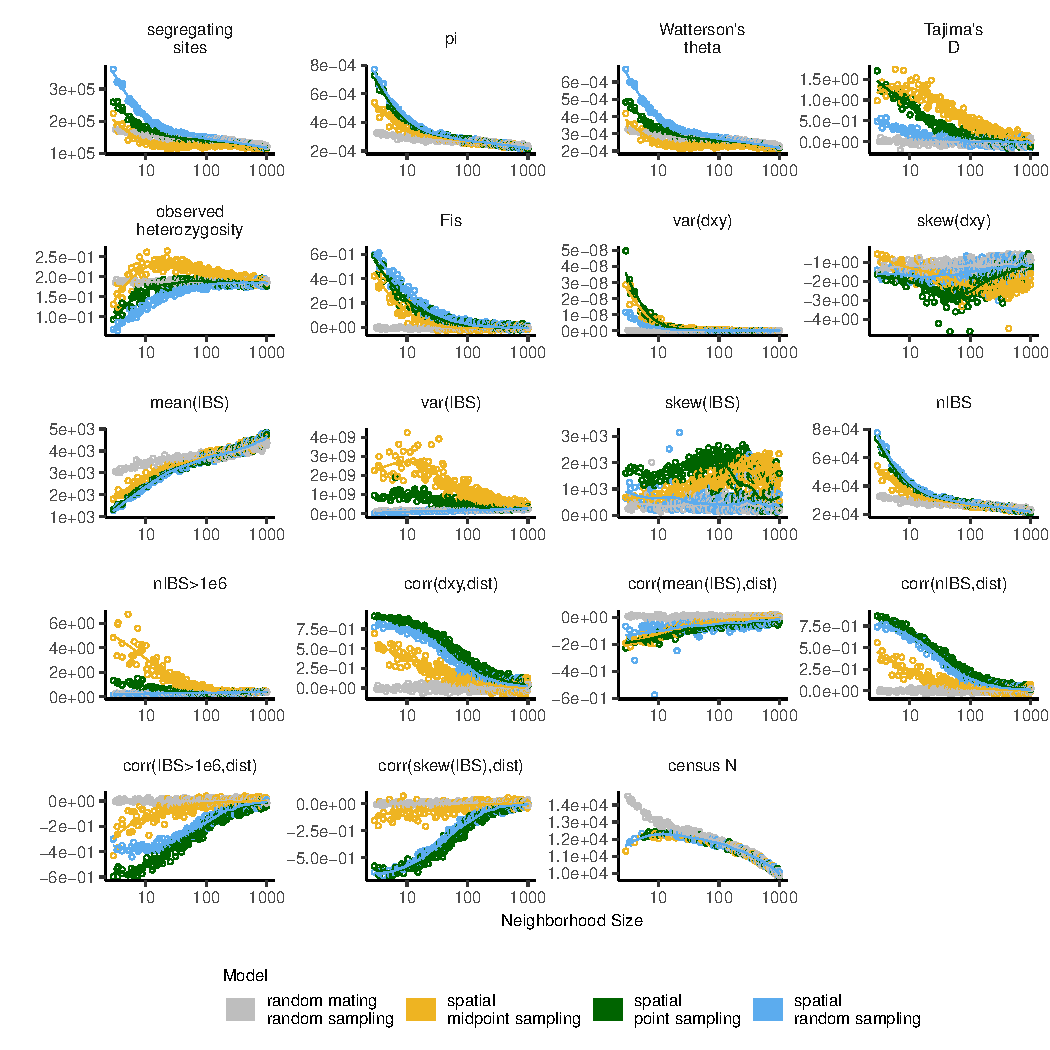
\includegraphics[width=\textwidth]{figures/sumstats_by_neighbors_allstats.pdf}
\caption{Change in summary statistics by neighborhood size and sampling scheme calculated from simulated sequence data of 60 individuals.}
\label{fig:allsumstats} 
\end{figure*}


\afterpage{\clearpage}
\begin{figure*}[p]
\centering
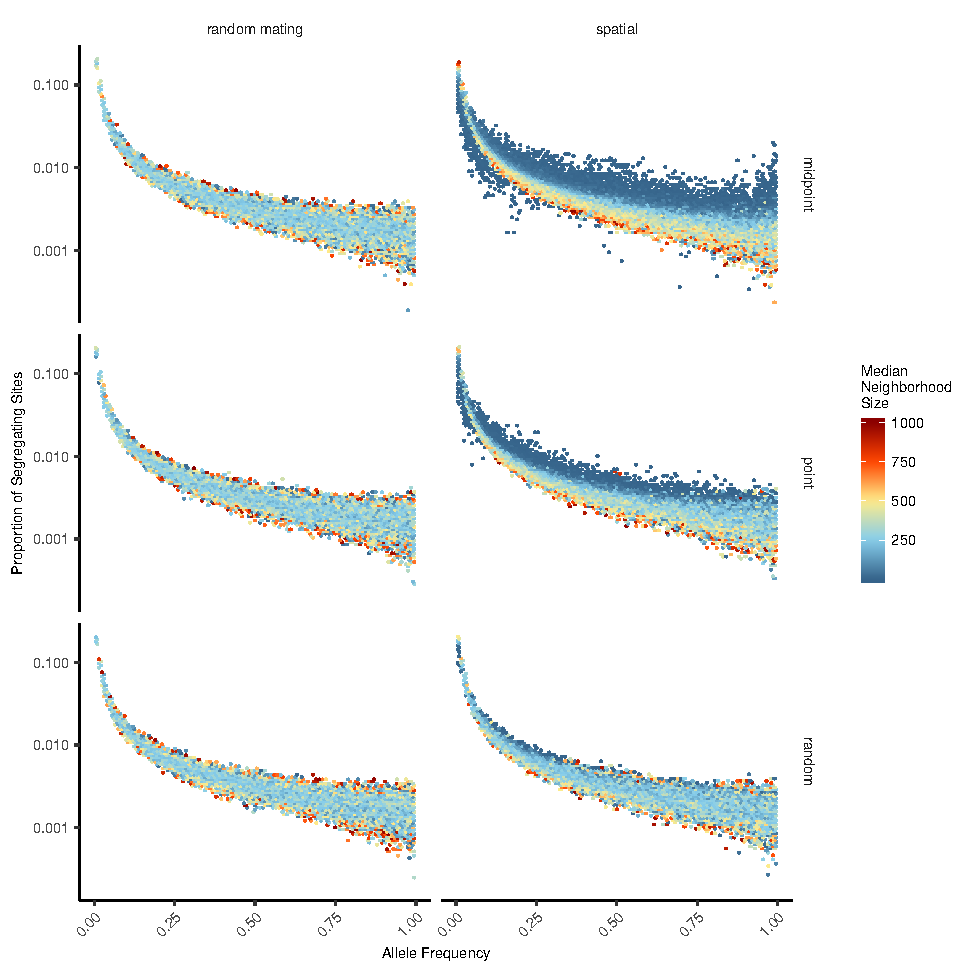
\includegraphics[width=\textwidth]{figures/fig_S1_sfs_grid_model_by_sampling.pdf}
\caption{Site frequency spectra for random mating and spatial SLiM models under all sampling schemes.}
\label{fig:allsfs}
\end{figure*}

\afterpage{\clearpage}
\begin{figure*}[p]
\centering
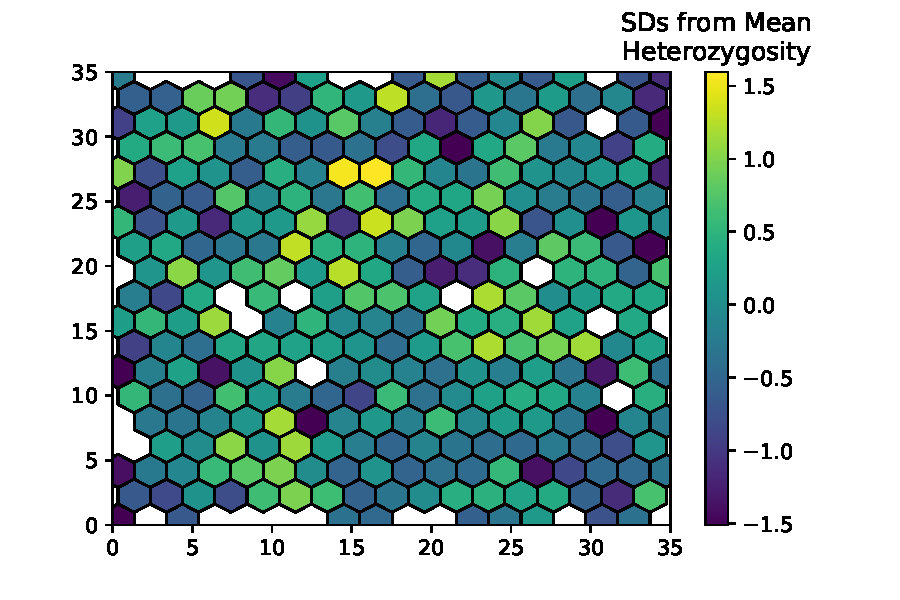
\includegraphics[]{figures/het_z_by_ind.pdf}
\caption{Normalized mean observed heterozygosity by location across 200 randomly-sampled individuals}
\label{fig:hetmap}
\end{figure*}


\begin{table}
\small
\centering
\caption{\bf Summary statistics calculated on simulated genotypes.}
\begin{tabular}{rllrrrrr}
  \hline
Statistic & Description \\ 
  \hline
$\Theta_{/pi}$ & Mean of the distribution of pairwise genetic differences \\
$\Theta_{/W}$ & Effective population size based on segregating sites \\
Segregating Sites & Total number of segregating sites in the sample \\
Tajima's $D$ & Difference in $\Theta_{/pi}$ and $\Theta_{/W}$ over its standard deviation\\
Observed Heterzygosity & Proportion of heterozygous individuals in the sample \\
$F_{is}$ & Wright's inbreeding coefficient $1-H_{e}/H_{o}$ \\
$var(D_{xy})$ & Variance in the distribution of pairwise genetic distances \\
$skew(D_{xy})$ & Skew of the distribution of pairwise genetic distances \\
$mean(IBS)$ & \makecell[l]{Mean of the distribution of pairwise identical-by-state (IBS) \\tract lengths taken over all pairs.} \\
$var(IBS)$ & \makecell[l]{Variance of the distribution of pairwise identical-by-state (IBS) \\tract lengths taken over all pairs.} \\
$skew(IBS)$ & \makecell[l]{Skew of the distribution of pairwise identical-by-state (IBS) \\tract lengths taken over all pairs.} \\
$nIBS$ & Number of IBS tracts with length > 2bp across all pairs of individuals. \\
$mean(IBS>1e6)$ & \makecell[l]{Mean number of IBS tracts over $1\times10^6$bp per pair \\across all pairs in the sample.} \\ 
$corr(D_{xy},dist)$ & Pearson correlation between genetic distance and $log_{10}(spatial\text{ }distance)$ \\
$corr(mean(IBS),dist)$ & \makecell[l]{Pearson correlation between the mean of the IBS tract distribution \\for each pair of samples and $log_{10}(spatial\text{ }distance)$} \\
$corr(nIBS,dist)$ & \makecell[l]{Pearson correlation between the number of IBS tracts \\for each pair of samples and $log_{10}(spatial\text{ }distance)$} \\
$corr(IBS>1e6,dist)$ & \makecell[l]{Pearson correlation between the number of IBS tracts $> 1\times10^6$bp \\for each pair of samples and $log_{10}(spatial\text{ }distance)$} \\
$corr(skew(IBS),dist)$ & \makecell[l]{Pearson correlation between the skew of the distribution of pairwise haplotype\\ block lengths for each pair of samples and $log_{10}(spatial\text{ }distance)$} \\
\end{tabular}
\label{table:sumstats}
\end{table}


\begin{table*}[htbp]
\tiny
\centering
\caption{\bf Anova and Levene's test $p$ values for differences by sampling strategy. Bolded values are rejected at \alpha=0.05}
\begin{tableminipage}{\textwidth}
\begin{tabularx}{\textwidth}{XXXX}
  \hline
 variable & model & p(equal means) & p(equal variance) \\ 
  \hline
segsites & random mating & 0.998190 & 0.980730 \\ 
pi & random mating & 0.997750 & 0.996450 \\ 
thetaW & random mating & 0.998190 & 0.980730 \\ 
tajD & random mating & 0.879690 & 0.188770 \\ 
het\_o & random mating & 0.531540 & 0.433230 \\ 
fis & random mating & 0.474790 & 0.785730 \\ 
gen\_dist\_mean & random mating & 0.997770 & 0.996510 \\ 
gen\_dist\_var & random mating & 0.283630 & 0.647240 \\ 
gen\_dist\_skew & random mating & 0.958320 & 0.260750 \\ 
gen\_sp\_corr & random mating & 0.601980 &\textbf{0.000000} \\ 
ibs\_mean & random mating & 0.997960 & 0.997730 \\ 
ibs\_var & random mating & 0.486450 & 0.399490 \\ 
ibs\_skew & random mating & 0.117980 & 0.069770 \\ 
ibs\_blocks\_per\_pair & random mating & 0.997680 & 0.996570 \\ 
ibs\_blocks\_over\_1e6\_per\_pair & random mating & 0.834870 & 0.888730 \\ 
ibs\_mean\_spat\_corr & random mating & 0.073270 & 0.308420 \\ 
ibs\_1e6blocks\_spat\_corr & random mating & 0.268440 & \textbf{0.002100} \\ 
ibs\_skew\_spat\_corr & random mating & 0.396920 & \textbf{0.000620} \\ 
ibs\_blocks\_spat\_corr & random mating & 0.581090 & \textbf{0.000000} \\ 
segsites & spatial & \textbf{0.000000} & \textbf{0.000000} \\ 
pi & spatial & \textbf{0.026510} & \textbf{0.013440} \\ 
thetaW & spatial & \textbf{0.000000} & \textbf{0.000000} \\ 
tajD & spatial & \textbf{0.000000} & \textbf{0.000000} \\ 
het\_o & spatial & \textbf{0.000000} & \textbf{0.000000} \\ 
fis & spatial & \textbf{0.000000} & \textbf{0.000120} \\ 
gen\_dist\_mean & spatial & \textbf{0.025390} & \textbf{0.012910} \\ 
gen\_dist\_var & spatial & \textbf{0.004970} & \textbf{0.006230} \\ 
gen\_dist\_skew & spatial & \textbf{0.000000} & \textbf{0.000000} \\ 
gen\_sp\_corr & spatial & \textbf{0.000000} & \textbf{0.000000} \\ 
ibs\_mean & spatial & 0.272400 & 0.114250 \\ 
ibs\_var & spatial & \textbf{0.000000} & \textbf{0.000000} \\ 
ibs\_skew & spatial & \textbf{0.000000} & \textbf{0.000000} \\ 
ibs\_blocks\_per\_pair & spatial & \textbf{0.033920} & \textbf{0.016640} \\ 
ibs\_blocks\_over\_1e6\_per\_pair & spatial & \textbf{0.000000} & \textbf{0.000000} \\ 
ibs\_mean\_spat\_corr & spatial & \textbf{0.000000} & 0.590540 \\ 
ibs\_1e6blocks\_spat\_corr & spatial & \textbf{0.000000} & \textbf{0.000000} \\ 
ibs\_skew\_spat\_corr & spatial & \textbf{0.000000} & \textbf{0.000000} \\ 
ibs\_blocks\_spat\_corr & spatial & \textbf{0.000000} & \textbf{0.000000} \\ 
\hline
\end{tabularx}
\end{tableminipage}
\label{table:sampling}
\end{table*}

% latex table generated in R 3.5.1 by xtable 1.8-3 package
% Fri Mar 22 13:50:47 2019
\begin{table}[ht]
\small
\centering
\caption{\bf T-test results comparing standard deviations of inferred $N_{e}$ between spatial and coalescent models, by neighborhood size (NS) and sampling strategy. $p$ is the probability that spatial models have higher standard deviations.}
\begin{tabular}{rllrrrrr}
  \hline
sampling & NS range & t & df & $p$ \\ 
  \hline
random & 2-20 & 4.2572 & 41.6166 & 0.0001 \\ 
random & 20-100 & -1.8473 & 171.9905 & 0.9668 \\ 
random & 100-500 & -2.1297 & 164.3864  & 0.9827 \\ 
random & 500-1000 & -3.9681 & 147.0497 & 0.9999 \\ 
point & 2-20 & 7.0802 & 44.3615  & 0.0000 \\ 
point & 20-100 & -0.2038 & 169.3799 & 0.5806 \\ 
point & 100-500 & -2.4945 & 152.5000 & 0.9932 \\ 
point & 500-1000 & -3.8329 & 162.6443& 0.9999 \\ 
midpoint & 2-20 & 5.9253 & 59.5462 & 0.0000 \\ 
midpoint & 20-100 & 3.8940 & 171.7005  & 0.0001 \\ 
midpoint & 100-500 & -2.2764 & 139.5221 & 0.9878 \\ 
midpoint & 500-1000 & -3.2223 & 165.0792 & 0.9992 \\ 
   \hline
\end{tabular}
\label{table:demography}
\end{table}


\stopsupplement



\end{document}

